\documentclass[11pt,a4paper]{article}
\usepackage[margin=25mm]{geometry}
\usepackage{amsmath,amssymb,amsthm,booktabs,array}
\usepackage[T1]{fontenc}
\usepackage{lmodern}
\usepackage[british]{babel}
\usepackage{tikz}
\usepackage{xurl}
\usepackage[colorlinks=true,linkcolor=blue,urlcolor=blue,citecolor=blue]{hyperref}
\hypersetup{
  pdftitle={A 180-vertex non-Rupert polyhedron with icosahedral symmetry},
  pdfauthor={Valentin Comte},
  pdfsubject={Convex geometry and formal verification},
  pdfkeywords={Rupert's problem, polyhedra, icosahedral symmetry, Lean}}
\newtheorem{theorem}{Theorem}
\newtheorem{lemma}[theorem]{Lemma}
\newtheorem{proposition}[theorem]{Proposition}
\newcommand{\conv}{\operatorname{conv}}
\newcommand{\intr}{\operatorname{int}}
\newcommand{\SO}{\operatorname{SO}}
\newcommand{\Q}{\mathbb Q}
\newcommand{\R}{\mathbb R}
\newcommand{\HH}{H}
\title{A 180-vertex non-Rupert polyhedron\\with icosahedral symmetry}
\author{Valentin Comte}
\date{17 November 2026}
\begin{document}
\maketitle
\begin{abstract}
We construct a centrally symmetric convex polyhedron with 180 vertices in
$\Q(\sqrt5)^3$ and give a computer-assisted proof that it does not have
Rupert's property. The body is the convex hull of two orbits under the full
icosahedral group. Symmetry reduces the passage problem to a compact
five-dimensional domain. Exact supporting inequalities exclude its regular
regions; divided finite-rotation inequalities and reflection transport handle
neighbourhoods where the shadows touch. A complete certificate covers all
432 initial regions. A subsequent Lean 4.19 formalisation establishes the
global strict-shadow noncontainment theorem; its retained final audit reports
only propositional extensionality, classical choice and quotient soundness.
We describe the geometric argument, its finite checks and the assumptions on
the implementations. Portable distribution and independent reproduction of
the large generated Lean corpus are distinguished from the completed research run.
\end{abstract}

\section{Introduction}
A convex body has \emph{Rupert's property} if a congruent copy can pass,
without turning, through a straight tunnel in it with positive clearance.
Equivalently, two suitably oriented copies have planar orthogonal projections
with one strictly contained in the other, allowing a translation in the
projection plane \cite{SYalgorithm}. Equality of shadows is not a passage.
We consider this straight-passage problem throughout.

Steininger and Yurkevich constructed the 90-vertex Noperthedron, disproving
the conjecture that every convex polyhedron is Rupert \cite{SYnopert}.
Subsequent public proofs address the rhombicosidodecahedron (RID)
\cite{Hervay,Smith,Jung}. Murphy's recent work reports further examples,
including the seven-vertex Septopert, and a Lean proof that every convex
polyhedron with at most six vertices is Rupert \cite{Murphy}.
Our aim is not to minimise the vertex count, but to give a further explicit
construction whose contact obstructions can be examined exactly.

The proof follows the certificate approach of these works. Its main
difficulty is not a lack of numerical resolution: at certain configurations,
the two shadows touch and a uniform strict separating margin vanishes.
The remedy is to retain the exact finite-rotation polynomial, divide out
known contact factors, and treat their zero sets separately. The contribution
here is the particular two-orbit body and its body-specific contact and
coverage certificates. We do not claim new general principles of symmetry
reduction, support separation or polynomial sign testing.

\section{The solid and the theorem}\label{sec:solid}
Put $\varphi=(1+\sqrt5)/2$. Fix the coordinate frame by taking $I\subset\SO(3)$
to be the rotation group preserving the 12 points obtained from
$(0,\varphi,1)$ by cyclic coordinate permutations and independent sign changes.
For real $a,b$, define
\[
 K(a,b)=\conv\{\pm g(2+\varphi+a,b,\varphi^2):g\in I\}.
\]
The particular body studied here is
\begin{equation}\label{eq:body}
 \HH=\conv\left(K(-\tfrac14,0)\ \cup\ \tfrac{19}{20}K(0,\tfrac1{10})\right).
\end{equation}
Equivalently, take the two generating points
$(\varphi+7/4,0,\varphi^2)$ and
$(19/20)(2+\varphi,1/10,\varphi^2)$, apply the group $I\cup(-I)$ to each,
and take the convex hull of the resulting points.

Central symmetry and invariance under $I$ follow directly from the definition.
Set $x=\varphi+7/4$ and $z=\varphi^2$. The first orbit contains
$(x,0,z),(z,x,0),(0,z,x)$ and their negatives. The determinant of these three
vectors is $x^3+z^3>0$, so $\HH$ is full-dimensional and the origin is interior.
The two generating sets have 60 and 120 distinct points respectively. The
geometric certificate verifies their disjointness and a strictly exposing
linear functional for each point. Hence $\HH$ has exactly 180 vertices, all
in $\Q(\sqrt5)^3$. A complete enumeration of its faces is unnecessary.

\begin{figure}[htbp]
\centering
% Generated from the frozen vertices by manuscript_assets/export_solid.py.
% BEGIN exact-coordinate solid illustration
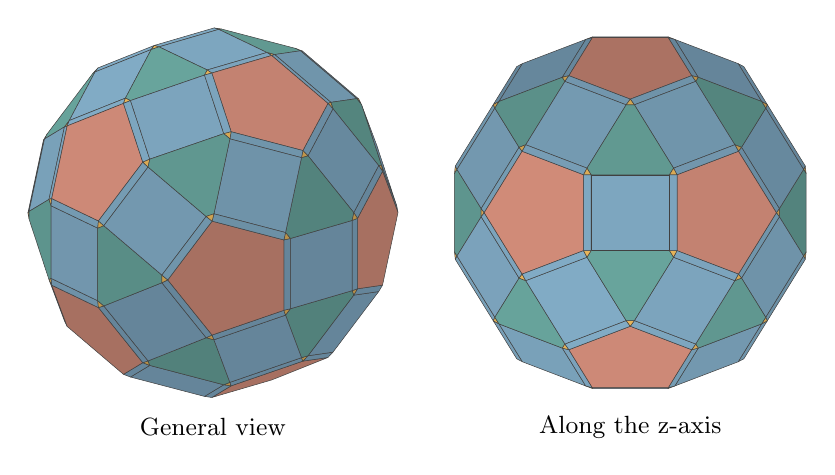
\begin{tikzpicture}[x=1cm,y=1cm,line join=round,line cap=round]
\definecolor{solidFace3}{RGB}{234,183,91}
\definecolor{solidFace4}{RGB}{129,171,197}
\definecolor{solidFace5}{RGB}{214,143,124}
\definecolor{solidFace6}{RGB}{105,166,158}
\path[fill=solidFace3!96!black,draw=black!75,line width=.18pt] (-4.80356,0.92007) -- (-4.78958,0.93657) -- (-4.75507,1.00154) -- cycle;
\path[fill=solidFace3!90!black,draw=black!75,line width=.18pt] (-1.53811,2.05612) -- (-1.51351,2.05291) -- (-1.60255,2.08702) -- cycle;
\path[fill=solidFace4!93!black,draw=black!75,line width=.18pt] (-4.99999,-0.00217) -- (-4.98559,0.01628) -- (-4.78958,0.93657) -- (-4.80356,0.92007) -- cycle;
\path[fill=solidFace4!86!black,draw=black!75,line width=.18pt] (-1.53811,2.05612) -- (-0.82470,1.44897) -- (-0.79858,1.44446) -- (-1.51351,2.05291) -- cycle;
\path[fill=solidFace4!78!black,draw=black!75,line width=.18pt] (-0.76355,1.37298) -- (-0.51042,0.60368) -- (-0.31441,0.08076) -- (-0.56754,0.85006) -- cycle;
\path[fill=solidFace3!89!black,draw=black!75,line width=.18pt] (-4.98559,-0.08076) -- (-4.98559,0.01628) -- (-4.99999,-0.00217) -- cycle;
\path[fill=solidFace3!98!black,draw=black!75,line width=.18pt] (-4.17412,1.77136) -- (-4.14748,1.78743) -- (-4.11012,1.83896) -- cycle;
\path[fill=solidFace3!80!black,draw=black!75,line width=.18pt] (-0.82470,1.44897) -- (-0.76355,1.37298) -- (-0.79858,1.44446) -- cycle;
\path[fill=solidFace3!94!black,draw=black!75,line width=.18pt] (-2.57706,2.32816) -- (-2.54255,2.33315) -- (-2.63552,2.34670) -- cycle;
\path[fill=solidFace5!78!black,draw=black!75,line width=.18pt] (-1.18988,-1.83896) -- (-1.50771,-1.88491) -- (-2.41906,-2.19871) -- (-2.66448,-2.34670) -- (-1.90480,-2.12436) -- cycle;
\path[fill=solidFace4!81!black,draw=black!75,line width=.18pt] (-4.50142,-1.44446) -- (-4.69785,-0.92044) -- (-4.73246,-0.85006) -- (-4.53645,-1.37298) -- cycle;
\path[fill=solidFace6!98!black,draw=black!75,line width=.18pt] (-4.78958,0.93657) -- (-4.53645,1.08921) -- (-4.47530,1.17025) -- (-4.14748,1.78743) -- (-4.17412,1.77136) -- (-4.75507,1.00154) -- cycle;
\path[fill=solidFace6!92!black,draw=black!75,line width=.18pt] (-1.96488,2.03464) -- (-1.86593,2.00873) -- (-1.53811,2.05612) -- (-1.60255,2.08702) -- (-2.54255,2.33315) -- (-2.57706,2.32816) -- cycle;
\path[fill=solidFace4!78!black,draw=black!75,line width=.18pt] (-2.66448,-2.34670) -- (-2.41906,-2.19871) -- (-2.51255,-2.18548) -- (-2.75745,-2.33315) -- cycle;
\path[fill=solidFace4!78!black,draw=black!75,line width=.18pt] (-0.51042,0.60368) -- (-0.49644,0.52620) -- (-0.30001,0.00217) -- (-0.31441,0.08076) -- cycle;
\path[fill=solidFace4!78!black,draw=black!75,line width=.18pt] (-1.12588,-1.77136) -- (-1.44303,-1.81722) -- (-1.50771,-1.88491) -- (-1.18988,-1.83896) -- cycle;
\path[fill=solidFace4!100!black,draw=black!75,line width=.18pt] (-4.14748,1.78743) -- (-3.43407,2.07222) -- (-3.39520,2.12436) -- (-4.11012,1.83896) -- cycle;
\path[fill=solidFace4!98!black,draw=black!75,line width=.18pt] (-3.39520,2.12436) -- (-3.33512,2.10629) -- (-2.57706,2.32816) -- (-2.63552,2.34670) -- cycle;
\path[fill=solidFace4!78!black,draw=black!75,line width=.18pt] (-2.75745,-2.33315) -- (-2.51255,-2.18548) -- (-3.45255,-1.93935) -- (-3.69745,-2.08702) -- cycle;
\path[fill=solidFace4!94!black,draw=black!75,line width=.18pt] (-4.98559,0.01628) -- (-4.73246,0.16892) -- (-4.53645,1.08921) -- (-4.78958,0.93657) -- cycle;
\path[fill=solidFace4!78!black,draw=black!75,line width=.18pt] (-0.54493,-1.00154) -- (-0.86208,-1.04739) -- (-1.44303,-1.81722) -- (-1.12588,-1.77136) -- cycle;
\path[fill=solidFace4!87!black,draw=black!75,line width=.18pt] (-1.86593,2.00873) -- (-1.15252,1.40157) -- (-0.82470,1.44897) -- (-1.53811,2.05612) -- cycle;
\path[fill=solidFace4!78!black,draw=black!75,line width=.18pt] (-3.69745,-2.08702) -- (-3.45255,-1.93935) -- (-3.54107,-1.90492) -- (-3.78649,-2.05291) -- cycle;
\path[fill=solidFace6!89!black,draw=black!75,line width=.18pt] (-4.73246,-0.85006) -- (-4.70582,-0.83400) -- (-4.70582,0.08794) -- (-4.73246,0.16892) -- (-4.98559,0.01628) -- (-4.98559,-0.08076) -- cycle;
\path[fill=solidFace5!78!black,draw=black!75,line width=.18pt] (-3.78649,-2.05291) -- (-3.54107,-1.90492) -- (-4.10432,-1.20502) -- (-4.69785,-0.92044) -- (-4.50142,-1.44446) -- cycle;
\path[fill=solidFace4!78!black,draw=black!75,line width=.18pt] (-0.49644,-0.92007) -- (-0.81427,-0.96603) -- (-0.86208,-1.04739) -- (-0.54493,-1.00154) -- cycle;
\path[fill=solidFace3!87!black,draw=black!75,line width=.18pt] (-4.69785,-0.92044) -- (-4.70582,-0.83400) -- (-4.73246,-0.85006) -- cycle;
\path[fill=solidFace6!80!black,draw=black!75,line width=.18pt] (-1.15252,1.40157) -- (-1.12588,1.32059) -- (-0.54493,0.59869) -- (-0.51042,0.60368) -- (-0.76355,1.37298) -- (-0.82470,1.44897) -- cycle;
\path[fill=solidFace5!78!black,draw=black!75,line width=.18pt] (-0.49644,0.52620) -- (-0.81427,-0.07218) -- (-0.81427,-0.96603) -- (-0.49644,-0.92007) -- (-0.30001,0.00217) -- cycle;
\path[fill=solidFace3!99!black,draw=black!75,line width=.18pt] (-3.43407,2.07222) -- (-3.33512,2.10629) -- (-3.39520,2.12436) -- cycle;
\path[fill=solidFace3!78!black,draw=black!75,line width=.18pt] (-0.54493,0.59869) -- (-0.49644,0.52620) -- (-0.51042,0.60368) -- cycle;
\path[fill=solidFace4!100!black,draw=black!75,line width=.18pt] (-4.47530,1.17025) -- (-3.76189,1.45504) -- (-3.43407,2.07222) -- (-4.14748,1.78743) -- cycle;
\path[fill=solidFace3!78!black,draw=black!75,line width=.18pt] (-2.41906,-2.19871) -- (-2.43493,-2.15449) -- (-2.51255,-2.18548) -- cycle;
\path[fill=solidFace4!97!black,draw=black!75,line width=.18pt] (-2.72294,1.81277) -- (-1.96488,2.03464) -- (-2.57706,2.32816) -- (-3.33512,2.10629) -- cycle;
\path[fill=solidFace4!78!black,draw=black!75,line width=.18pt] (-1.50771,-1.88491) -- (-1.52551,-1.84136) -- (-2.43493,-2.15449) -- (-2.41906,-2.19871) -- cycle;
\path[fill=solidFace3!78!black,draw=black!75,line width=.18pt] (-1.44303,-1.81722) -- (-1.52551,-1.84136) -- (-1.50771,-1.88491) -- cycle;
\path[fill=solidFace3!98!black,draw=black!75,line width=.18pt] (-4.53645,1.08921) -- (-4.50142,1.10227) -- (-4.47530,1.17025) -- cycle;
\path[fill=solidFace3!93!black,draw=black!75,line width=.18pt] (-1.96488,2.03464) -- (-1.90480,1.99634) -- (-1.86593,2.00873) -- cycle;
\path[fill=solidFace4!95!black,draw=black!75,line width=.18pt] (-4.73246,0.16892) -- (-4.69785,0.18002) -- (-4.50142,1.10227) -- (-4.53645,1.08921) -- cycle;
\path[fill=solidFace4!88!black,draw=black!75,line width=.18pt] (-1.90480,1.99634) -- (-1.18988,1.38789) -- (-1.15252,1.40157) -- (-1.86593,2.00873) -- cycle;
\path[fill=solidFace3!78!black,draw=black!75,line width=.18pt] (-3.45255,-1.93935) -- (-3.47388,-1.88245) -- (-3.54107,-1.90492) -- cycle;
\path[fill=solidFace4!85!black,draw=black!75,line width=.18pt] (-4.10432,-1.20502) -- (-4.11355,-1.11797) -- (-4.70582,-0.83400) -- (-4.69785,-0.92044) -- cycle;
\path[fill=solidFace3!91!black,draw=black!75,line width=.18pt] (-4.70582,0.08794) -- (-4.69785,0.18002) -- (-4.73246,0.16892) -- cycle;
\path[fill=solidFace3!78!black,draw=black!75,line width=.18pt] (-0.81427,-0.96603) -- (-0.88341,-0.99050) -- (-0.86208,-1.04739) -- cycle;
\path[fill=solidFace4!78!black,draw=black!75,line width=.18pt] (-0.86208,0.00158) -- (-0.81427,-0.07218) -- (-0.49644,0.52620) -- (-0.54493,0.59869) -- cycle;
\path[fill=solidFace3!82!black,draw=black!75,line width=.18pt] (-1.18988,1.38789) -- (-1.12588,1.32059) -- (-1.15252,1.40157) -- cycle;
\path[fill=solidFace4!100!black,draw=black!75,line width=.18pt] (-4.50142,1.10227) -- (-3.78649,1.38767) -- (-3.76189,1.45504) -- (-4.47530,1.17025) -- cycle;
\path[fill=solidFace6!78!black,draw=black!75,line width=.18pt] (-2.51255,-2.18548) -- (-2.43493,-2.15449) -- (-2.63754,-1.61399) -- (-2.73648,-1.58809) -- (-3.47388,-1.88245) -- (-3.45255,-1.93935) -- cycle;
\path[fill=solidFace4!96!black,draw=black!75,line width=.18pt] (-2.66448,1.77400) -- (-1.90480,1.99634) -- (-1.96488,2.03464) -- (-2.72294,1.81277) -- cycle;
\path[fill=solidFace6!78!black,draw=black!75,line width=.18pt] (-0.86208,-1.04739) -- (-0.88341,-0.99050) -- (-1.66696,-1.21983) -- (-1.72811,-1.30086) -- (-1.52551,-1.84136) -- (-1.44303,-1.81722) -- cycle;
\path[fill=solidFace6!99!black,draw=black!75,line width=.18pt] (-3.69745,1.42414) -- (-2.75745,1.74780) -- (-2.72294,1.81277) -- (-3.33512,2.10629) -- (-3.43407,2.07222) -- (-3.76189,1.45504) -- cycle;
\path[fill=solidFace4!78!black,draw=black!75,line width=.18pt] (-3.54107,-1.90492) -- (-3.47388,-1.88245) -- (-4.03593,-1.18403) -- (-4.10432,-1.20502) -- cycle;
\path[fill=solidFace4!88!black,draw=black!75,line width=.18pt] (-4.11355,-1.11797) -- (-4.11355,-0.19603) -- (-4.70582,0.08794) -- (-4.70582,-0.83400) -- cycle;
\path[fill=solidFace4!78!black,draw=black!75,line width=.18pt] (-1.52551,-1.84136) -- (-1.72811,-1.30086) -- (-2.63754,-1.61399) -- (-2.43493,-2.15449) -- cycle;
\path[fill=solidFace4!78!black,draw=black!75,line width=.18pt] (-0.81427,-0.07218) -- (-0.88341,-0.09855) -- (-0.88341,-0.99050) -- (-0.81427,-0.96603) -- cycle;
\path[fill=solidFace4!80!black,draw=black!75,line width=.18pt] (-1.44303,0.72348) -- (-0.86208,0.00158) -- (-0.54493,0.59869) -- (-1.12588,1.32059) -- cycle;
\path[fill=solidFace3!83!black,draw=black!75,line width=.18pt] (-4.10432,-1.20502) -- (-4.03593,-1.18403) -- (-4.11355,-1.11797) -- cycle;
\path[fill=solidFace4!90!black,draw=black!75,line width=.18pt] (-4.11355,-0.19603) -- (-4.10432,-0.10456) -- (-4.69785,0.18002) -- (-4.70582,0.08794) -- cycle;
\path[fill=solidFace3!78!black,draw=black!75,line width=.18pt] (-0.88341,-0.09855) -- (-0.81427,-0.07218) -- (-0.86208,0.00158) -- cycle;
\path[fill=solidFace3!99!black,draw=black!75,line width=.18pt] (-3.78649,1.38767) -- (-3.69745,1.42414) -- (-3.76189,1.45504) -- cycle;
\path[fill=solidFace5!96!black,draw=black!75,line width=.18pt] (-4.10432,-0.10456) -- (-3.54107,0.64181) -- (-3.78649,1.38767) -- (-4.50142,1.10227) -- (-4.69785,0.18002) -- cycle;
\path[fill=solidFace3!98!black,draw=black!75,line width=.18pt] (-2.75745,1.74780) -- (-2.66448,1.77400) -- (-2.72294,1.81277) -- cycle;
\path[fill=solidFace4!82!black,draw=black!75,line width=.18pt] (-1.50771,0.78951) -- (-1.44303,0.72348) -- (-1.12588,1.32059) -- (-1.18988,1.38789) -- cycle;
\path[fill=solidFace5!91!black,draw=black!75,line width=.18pt] (-2.41906,1.02814) -- (-1.50771,0.78951) -- (-1.18988,1.38789) -- (-1.90480,1.99634) -- (-2.66448,1.77400) -- cycle;
\path[fill=solidFace4!78!black,draw=black!75,line width=.18pt] (-3.47388,-1.88245) -- (-2.73648,-1.58809) -- (-3.29854,-0.88966) -- (-4.03593,-1.18403) -- cycle;
\path[fill=solidFace4!78!black,draw=black!75,line width=.18pt] (-0.88341,-0.99050) -- (-0.88341,-0.09855) -- (-1.66696,-0.32788) -- (-1.66696,-1.21983) -- cycle;
\path[fill=solidFace3!78!black,draw=black!75,line width=.18pt] (-2.63754,-1.61399) -- (-2.66090,-1.55356) -- (-2.73648,-1.58809) -- cycle;
\path[fill=solidFace4!78!black,draw=black!75,line width=.18pt] (-1.72811,-1.30086) -- (-1.74954,-1.23976) -- (-2.66090,-1.55356) -- (-2.63754,-1.61399) -- cycle;
\path[fill=solidFace3!78!black,draw=black!75,line width=.18pt] (-1.66696,-1.21983) -- (-1.74954,-1.23976) -- (-1.72811,-1.30086) -- cycle;
\path[fill=solidFace6!85!black,draw=black!75,line width=.18pt] (-4.03593,-1.18403) -- (-3.29854,-0.88966) -- (-3.29854,-0.79262) -- (-4.03593,-0.16505) -- (-4.11355,-0.19603) -- (-4.11355,-1.11797) -- cycle;
\path[fill=solidFace4!97!black,draw=black!75,line width=.18pt] (-3.54107,0.64181) -- (-3.45255,0.67986) -- (-3.69745,1.42414) -- (-3.78649,1.38767) -- cycle;
\path[fill=solidFace4!96!black,draw=black!75,line width=.18pt] (-3.45255,0.67986) -- (-2.51255,1.00353) -- (-2.75745,1.74780) -- (-3.69745,1.42414) -- cycle;
\path[fill=solidFace4!96!black,draw=black!75,line width=.18pt] (-2.51255,1.00353) -- (-2.41906,1.02814) -- (-2.66448,1.77400) -- (-2.75745,1.74780) -- cycle;
\path[fill=solidFace6!79!black,draw=black!75,line width=.18pt] (-1.72811,-0.25189) -- (-1.66696,-0.32788) -- (-0.88341,-0.09855) -- (-0.86208,0.00158) -- (-1.44303,0.72348) -- (-1.52551,0.69934) -- cycle;
\path[fill=solidFace3!87!black,draw=black!75,line width=.18pt] (-4.11355,-0.19603) -- (-4.03593,-0.16505) -- (-4.10432,-0.10456) -- cycle;
\path[fill=solidFace3!82!black,draw=black!75,line width=.18pt] (-1.52551,0.69934) -- (-1.44303,0.72348) -- (-1.50771,0.78951) -- cycle;
\path[fill=solidFace4!78!black,draw=black!75,line width=.18pt] (-2.73648,-1.58809) -- (-2.66090,-1.55356) -- (-3.22414,-0.85365) -- (-3.29854,-0.88966) -- cycle;
\path[fill=solidFace4!78!black,draw=black!75,line width=.18pt] (-1.74954,-1.23976) -- (-1.66696,-1.21983) -- (-1.66696,-0.32788) -- (-1.74954,-0.34591) -- cycle;
\path[fill=solidFace4!91!black,draw=black!75,line width=.18pt] (-4.03593,-0.16505) -- (-3.47388,0.57974) -- (-3.54107,0.64181) -- (-4.10432,-0.10456) -- cycle;
\path[fill=solidFace4!87!black,draw=black!75,line width=.18pt] (-2.43493,0.93747) -- (-1.52551,0.69934) -- (-1.50771,0.78951) -- (-2.41906,1.02814) -- cycle;
\path[fill=solidFace5!78!black,draw=black!75,line width=.18pt] (-2.66090,-1.55356) -- (-1.74954,-1.23976) -- (-1.74954,-0.34591) -- (-2.66090,-0.10728) -- (-3.22414,-0.85365) -- cycle;
\path[fill=solidFace3!93!black,draw=black!75,line width=.18pt] (-3.47388,0.57974) -- (-3.45255,0.67986) -- (-3.54107,0.64181) -- cycle;
\path[fill=solidFace3!84!black,draw=black!75,line width=.18pt] (-3.29854,-0.88966) -- (-3.22414,-0.85365) -- (-3.29854,-0.79262) -- cycle;
\path[fill=solidFace4!89!black,draw=black!75,line width=.18pt] (-3.29854,-0.79262) -- (-2.73648,-0.04783) -- (-3.47388,0.57974) -- (-4.03593,-0.16505) -- cycle;
\path[fill=solidFace3!92!black,draw=black!75,line width=.18pt] (-2.43493,0.93747) -- (-2.41906,1.02814) -- (-2.51255,1.00353) -- cycle;
\path[fill=solidFace3!79!black,draw=black!75,line width=.18pt] (-1.74954,-0.34591) -- (-1.66696,-0.32788) -- (-1.72811,-0.25189) -- cycle;
\path[fill=solidFace4!86!black,draw=black!75,line width=.18pt] (-2.63754,-0.01376) -- (-1.72811,-0.25189) -- (-1.52551,0.69934) -- (-2.43493,0.93747) -- cycle;
\path[fill=solidFace6!91!black,draw=black!75,line width=.18pt] (-2.73648,-0.04783) -- (-2.63754,-0.01376) -- (-2.43493,0.93747) -- (-2.51255,1.00353) -- (-3.45255,0.67986) -- (-3.47388,0.57974) -- cycle;
\path[fill=solidFace4!87!black,draw=black!75,line width=.18pt] (-3.22414,-0.85365) -- (-2.66090,-0.10728) -- (-2.73648,-0.04783) -- (-3.29854,-0.79262) -- cycle;
\path[fill=solidFace4!84!black,draw=black!75,line width=.18pt] (-2.66090,-0.10728) -- (-1.74954,-0.34591) -- (-1.72811,-0.25189) -- (-2.63754,-0.01376) -- cycle;
\path[fill=solidFace3!89!black,draw=black!75,line width=.18pt] (-2.66090,-0.10728) -- (-2.63754,-0.01376) -- (-2.73648,-0.04783) -- cycle;
\node[font=\small] at (-2.650,-2.72) {General view};
\path[fill=solidFace4!79!black,draw=black!75,line width=.18pt] (0.98261,1.41246) -- (1.27988,1.89346) -- (1.20777,1.85539) -- (0.90986,1.37337) -- cycle;
\path[fill=solidFace4!78!black,draw=black!75,line width=.18pt] (4.31739,1.41246) -- (4.39014,1.37337) -- (4.09223,1.85539) -- (4.02012,1.89346) -- cycle;
\path[fill=solidFace4!93!black,draw=black!75,line width=.18pt] (1.20777,-1.85539) -- (1.27988,-1.89346) -- (0.98261,-1.41246) -- (0.90986,-1.37337) -- cycle;
\path[fill=solidFace4!87!black,draw=black!75,line width=.18pt] (4.09223,-1.85539) -- (4.39014,-1.37337) -- (4.31739,-1.41246) -- (4.02012,-1.89346) -- cycle;
\path[fill=solidFace3!88!black,draw=black!75,line width=.18pt] (0.41693,0.49717) -- (0.44928,0.54951) -- (0.42784,0.59344) -- cycle;
\path[fill=solidFace3!78!black,draw=black!75,line width=.18pt] (4.88307,0.49717) -- (4.87216,0.59344) -- (4.85072,0.54951) -- cycle;
\path[fill=solidFace3!90!black,draw=black!75,line width=.18pt] (0.42784,-0.59344) -- (0.44928,-0.54951) -- (0.41693,-0.49717) -- cycle;
\path[fill=solidFace3!79!black,draw=black!75,line width=.18pt] (4.87216,-0.59344) -- (4.88307,-0.49717) -- (4.85072,-0.54951) -- cycle;
\path[fill=solidFace4!78!black,draw=black!75,line width=.18pt] (3.13202,2.22216) -- (3.13100,2.23307) -- (2.16900,2.23307) -- (2.16798,2.22216) -- cycle;
\path[fill=solidFace4!90!black,draw=black!75,line width=.18pt] (3.13100,-2.23307) -- (3.13202,-2.22216) -- (2.16798,-2.22216) -- (2.16900,-2.23307) -- cycle;
\path[fill=solidFace3!78!black,draw=black!75,line width=.18pt] (2.16798,2.22216) -- (2.16900,2.23307) -- (2.08432,2.20072) -- cycle;
\path[fill=solidFace3!78!black,draw=black!75,line width=.18pt] (3.13202,2.22216) -- (3.21568,2.20072) -- (3.13100,2.23307) -- cycle;
\path[fill=solidFace3!91!black,draw=black!75,line width=.18pt] (2.16900,-2.23307) -- (2.16798,-2.22216) -- (2.08432,-2.20072) -- cycle;
\path[fill=solidFace3!87!black,draw=black!75,line width=.18pt] (3.13100,-2.23307) -- (3.21568,-2.20072) -- (3.13202,-2.22216) -- cycle;
\path[fill=solidFace4!94!black,draw=black!75,line width=.18pt] (0.90986,-1.37337) -- (0.93027,-1.32778) -- (0.44928,-0.54951) -- (0.42784,-0.59344) -- cycle;
\path[fill=solidFace4!87!black,draw=black!75,line width=.18pt] (0.44928,0.54951) -- (0.93027,1.32778) -- (0.90986,1.37337) -- (0.42784,0.59344) -- cycle;
\path[fill=solidFace4!84!black,draw=black!75,line width=.18pt] (4.39014,-1.37337) -- (4.87216,-0.59344) -- (4.85072,-0.54951) -- (4.36973,-1.32778) -- cycle;
\path[fill=solidFace4!78!black,draw=black!75,line width=.18pt] (4.85072,0.54951) -- (4.87216,0.59344) -- (4.39014,1.37337) -- (4.36973,1.32778) -- cycle;
\path[fill=solidFace4!79!black,draw=black!75,line width=.18pt] (1.78705,1.71973) -- (2.08432,2.20072) -- (1.27988,1.89346) -- (0.98261,1.41246) -- cycle;
\path[fill=solidFace4!78!black,draw=black!75,line width=.18pt] (3.51295,1.71973) -- (4.31739,1.41246) -- (4.02012,1.89346) -- (3.21568,2.20072) -- cycle;
\path[fill=solidFace4!94!black,draw=black!75,line width=.18pt] (1.27988,-1.89346) -- (2.08432,-2.20072) -- (1.78705,-1.71973) -- (0.98261,-1.41246) -- cycle;
\path[fill=solidFace4!89!black,draw=black!75,line width=.18pt] (4.02012,-1.89346) -- (4.31739,-1.41246) -- (3.51295,-1.71973) -- (3.21568,-2.20072) -- cycle;
\path[fill=solidFace6!90!black,draw=black!75,line width=.18pt] (0.44928,-0.54951) -- (0.75654,-0.05233) -- (0.75654,0.05233) -- (0.44928,0.54951) -- (0.41693,0.49717) -- (0.41693,-0.49717) -- cycle;
\path[fill=solidFace6!79!black,draw=black!75,line width=.18pt] (4.85072,-0.54951) -- (4.88307,-0.49717) -- (4.88307,0.49717) -- (4.85072,0.54951) -- (4.54346,0.05233) -- (4.54346,-0.05233) -- cycle;
\path[fill=solidFace3!85!black,draw=black!75,line width=.18pt] (0.93027,1.32778) -- (0.98261,1.41246) -- (0.90986,1.37337) -- cycle;
\path[fill=solidFace3!78!black,draw=black!75,line width=.18pt] (4.36973,1.32778) -- (4.39014,1.37337) -- (4.31739,1.41246) -- cycle;
\path[fill=solidFace3!96!black,draw=black!75,line width=.18pt] (0.90986,-1.37337) -- (0.98261,-1.41246) -- (0.93027,-1.32778) -- cycle;
\path[fill=solidFace3!89!black,draw=black!75,line width=.18pt] (4.39014,-1.37337) -- (4.36973,-1.32778) -- (4.31739,-1.41246) -- cycle;
\path[fill=solidFace4!79!black,draw=black!75,line width=.18pt] (1.87007,1.74014) -- (2.16798,2.22216) -- (2.08432,2.20072) -- (1.78705,1.71973) -- cycle;
\path[fill=solidFace4!78!black,draw=black!75,line width=.18pt] (3.42993,1.74014) -- (3.51295,1.71973) -- (3.21568,2.20072) -- (3.13202,2.22216) -- cycle;
\path[fill=solidFace4!91!black,draw=black!75,line width=.18pt] (3.21568,-2.20072) -- (3.51295,-1.71973) -- (3.42993,-1.74014) -- (3.13202,-2.22216) -- cycle;
\path[fill=solidFace4!95!black,draw=black!75,line width=.18pt] (2.08432,-2.20072) -- (2.16798,-2.22216) -- (1.87007,-1.74014) -- (1.78705,-1.71973) -- cycle;
\path[fill=solidFace4!89!black,draw=black!75,line width=.18pt] (0.75654,0.05233) -- (1.23754,0.83061) -- (0.93027,1.32778) -- (0.44928,0.54951) -- cycle;
\path[fill=solidFace4!86!black,draw=black!75,line width=.18pt] (4.36973,-1.32778) -- (4.85072,-0.54951) -- (4.54346,-0.05233) -- (4.06246,-0.83061) -- cycle;
\path[fill=solidFace4!80!black,draw=black!75,line width=.18pt] (4.54346,0.05233) -- (4.85072,0.54951) -- (4.36973,1.32778) -- (4.06246,0.83061) -- cycle;
\path[fill=solidFace4!95!black,draw=black!75,line width=.18pt] (0.93027,-1.32778) -- (1.23754,-0.83061) -- (0.75654,-0.05233) -- (0.44928,-0.54951) -- cycle;
\path[fill=solidFace5!80!black,draw=black!75,line width=.18pt] (2.65000,1.44223) -- (3.42993,1.74014) -- (3.13202,2.22216) -- (2.16798,2.22216) -- (1.87007,1.74014) -- cycle;
\path[fill=solidFace5!96!black,draw=black!75,line width=.18pt] (3.13202,-2.22216) -- (3.42993,-1.74014) -- (2.65000,-1.44223) -- (1.87007,-1.74014) -- (2.16798,-2.22216) -- cycle;
\path[fill=solidFace6!87!black,draw=black!75,line width=.18pt] (1.32222,0.86295) -- (1.81939,1.66739) -- (1.78705,1.71973) -- (0.98261,1.41246) -- (0.93027,1.32778) -- (1.23754,0.83061) -- cycle;
\path[fill=solidFace6!91!black,draw=black!75,line width=.18pt] (4.31739,-1.41246) -- (4.36973,-1.32778) -- (4.06246,-0.83061) -- (3.97778,-0.86295) -- (3.48061,-1.66739) -- (3.51295,-1.71973) -- cycle;
\path[fill=solidFace6!80!black,draw=black!75,line width=.18pt] (3.97778,0.86295) -- (4.06246,0.83061) -- (4.36973,1.32778) -- (4.31739,1.41246) -- (3.51295,1.71973) -- (3.48061,1.66739) -- cycle;
\path[fill=solidFace6!98!black,draw=black!75,line width=.18pt] (0.98261,-1.41246) -- (1.78705,-1.71973) -- (1.81939,-1.66739) -- (1.32222,-0.86295) -- (1.23754,-0.83061) -- (0.93027,-1.32778) -- cycle;
\path[fill=solidFace3!98!black,draw=black!75,line width=.18pt] (1.78705,-1.71973) -- (1.87007,-1.74014) -- (1.81939,-1.66739) -- cycle;
\path[fill=solidFace3!86!black,draw=black!75,line width=.18pt] (1.81939,1.66739) -- (1.87007,1.74014) -- (1.78705,1.71973) -- cycle;
\path[fill=solidFace3!93!black,draw=black!75,line width=.18pt] (3.51295,-1.71973) -- (3.48061,-1.66739) -- (3.42993,-1.74014) -- cycle;
\path[fill=solidFace3!80!black,draw=black!75,line width=.18pt] (3.48061,1.66739) -- (3.51295,1.71973) -- (3.42993,1.74014) -- cycle;
\path[fill=solidFace3!82!black,draw=black!75,line width=.18pt] (4.54346,-0.05233) -- (4.54346,0.05233) -- (4.50539,-0.00000) -- cycle;
\path[fill=solidFace3!92!black,draw=black!75,line width=.18pt] (0.75654,-0.05233) -- (0.79461,0.00000) -- (0.75654,0.05233) -- cycle;
\path[fill=solidFace4!96!black,draw=black!75,line width=.18pt] (1.23754,-0.83061) -- (1.27663,-0.77993) -- (0.79461,0.00000) -- (0.75654,-0.05233) -- cycle;
\path[fill=solidFace4!91!black,draw=black!75,line width=.18pt] (0.79461,0.00000) -- (1.27663,0.77993) -- (1.23754,0.83061) -- (0.75654,0.05233) -- cycle;
\path[fill=solidFace4!87!black,draw=black!75,line width=.18pt] (4.06246,-0.83061) -- (4.54346,-0.05233) -- (4.50539,-0.00000) -- (4.02337,-0.77993) -- cycle;
\path[fill=solidFace4!82!black,draw=black!75,line width=.18pt] (4.50539,-0.00000) -- (4.54346,0.05233) -- (4.06246,0.83061) -- (4.02337,0.77993) -- cycle;
\path[fill=solidFace4!100!black,draw=black!75,line width=.18pt] (1.87007,-1.74014) -- (2.65000,-1.44223) -- (2.59767,-1.37012) -- (1.81939,-1.66739) -- cycle;
\path[fill=solidFace4!88!black,draw=black!75,line width=.18pt] (2.59767,1.37012) -- (2.65000,1.44223) -- (1.87007,1.74014) -- (1.81939,1.66739) -- cycle;
\path[fill=solidFace4!97!black,draw=black!75,line width=.18pt] (3.42993,-1.74014) -- (3.48061,-1.66739) -- (2.70233,-1.37012) -- (2.65000,-1.44223) -- cycle;
\path[fill=solidFace4!86!black,draw=black!75,line width=.18pt] (2.70233,1.37012) -- (3.48061,1.66739) -- (3.42993,1.74014) -- (2.65000,1.44223) -- cycle;
\path[fill=solidFace3!98!black,draw=black!75,line width=.18pt] (1.23754,-0.83061) -- (1.32222,-0.86295) -- (1.27663,-0.77993) -- cycle;
\path[fill=solidFace3!89!black,draw=black!75,line width=.18pt] (1.27663,0.77993) -- (1.32222,0.86295) -- (1.23754,0.83061) -- cycle;
\path[fill=solidFace3!92!black,draw=black!75,line width=.18pt] (4.06246,-0.83061) -- (4.02337,-0.77993) -- (3.97778,-0.86295) -- cycle;
\path[fill=solidFace3!82!black,draw=black!75,line width=.18pt] (4.02337,0.77993) -- (4.06246,0.83061) -- (3.97778,0.86295) -- cycle;
\path[fill=solidFace4!100!black,draw=black!75,line width=.18pt] (1.81939,-1.66739) -- (2.59767,-1.37012) -- (2.10049,-0.56568) -- (1.32222,-0.86295) -- cycle;
\path[fill=solidFace4!90!black,draw=black!75,line width=.18pt] (2.10049,0.56568) -- (2.59767,1.37012) -- (1.81939,1.66739) -- (1.32222,0.86295) -- cycle;
\path[fill=solidFace4!96!black,draw=black!75,line width=.18pt] (3.48061,-1.66739) -- (3.97778,-0.86295) -- (3.19951,-0.56568) -- (2.70233,-1.37012) -- cycle;
\path[fill=solidFace4!87!black,draw=black!75,line width=.18pt] (3.19951,0.56568) -- (3.97778,0.86295) -- (3.48061,1.66739) -- (2.70233,1.37012) -- cycle;
\path[fill=solidFace5!97!black,draw=black!75,line width=.18pt] (1.27663,-0.77993) -- (2.05656,-0.48202) -- (2.05656,0.48202) -- (1.27663,0.77993) -- (0.79461,0.00000) -- cycle;
\path[fill=solidFace5!91!black,draw=black!75,line width=.18pt] (4.02337,-0.77993) -- (4.50539,-0.00000) -- (4.02337,0.77993) -- (3.24344,0.48202) -- (3.24344,-0.48202) -- cycle;
\path[fill=solidFace3!99!black,draw=black!75,line width=.18pt] (2.65000,-1.44223) -- (2.70233,-1.37012) -- (2.59767,-1.37012) -- cycle;
\path[fill=solidFace3!90!black,draw=black!75,line width=.18pt] (2.70233,1.37012) -- (2.65000,1.44223) -- (2.59767,1.37012) -- cycle;
\path[fill=solidFace4!92!black,draw=black!75,line width=.18pt] (2.05656,0.48202) -- (2.10049,0.56568) -- (1.32222,0.86295) -- (1.27663,0.77993) -- cycle;
\path[fill=solidFace4!96!black,draw=black!75,line width=.18pt] (3.97778,-0.86295) -- (4.02337,-0.77993) -- (3.24344,-0.48202) -- (3.19951,-0.56568) -- cycle;
\path[fill=solidFace4!88!black,draw=black!75,line width=.18pt] (3.24344,0.48202) -- (4.02337,0.77993) -- (3.97778,0.86295) -- (3.19951,0.56568) -- cycle;
\path[fill=solidFace4!100!black,draw=black!75,line width=.18pt] (1.32222,-0.86295) -- (2.10049,-0.56568) -- (2.05656,-0.48202) -- (1.27663,-0.77993) -- cycle;
\path[fill=solidFace6!99!black,draw=black!75,line width=.18pt] (2.70233,-1.37012) -- (3.19951,-0.56568) -- (3.14717,-0.48100) -- (2.15283,-0.48100) -- (2.10049,-0.56568) -- (2.59767,-1.37012) -- cycle;
\path[fill=solidFace6!92!black,draw=black!75,line width=.18pt] (3.14717,0.48100) -- (3.19951,0.56568) -- (2.70233,1.37012) -- (2.59767,1.37012) -- (2.10049,0.56568) -- (2.15283,0.48100) -- cycle;
\path[fill=solidFace3!99!black,draw=black!75,line width=.18pt] (2.10049,-0.56568) -- (2.15283,-0.48100) -- (2.05656,-0.48202) -- cycle;
\path[fill=solidFace3!94!black,draw=black!75,line width=.18pt] (2.15283,0.48100) -- (2.10049,0.56568) -- (2.05656,0.48202) -- cycle;
\path[fill=solidFace3!98!black,draw=black!75,line width=.18pt] (3.19951,-0.56568) -- (3.24344,-0.48202) -- (3.14717,-0.48100) -- cycle;
\path[fill=solidFace3!93!black,draw=black!75,line width=.18pt] (3.14717,0.48100) -- (3.24344,0.48202) -- (3.19951,0.56568) -- cycle;
\path[fill=solidFace4!98!black,draw=black!75,line width=.18pt] (2.05656,-0.48202) -- (2.15283,-0.48100) -- (2.15283,0.48100) -- (2.05656,0.48202) -- cycle;
\path[fill=solidFace4!96!black,draw=black!75,line width=.18pt] (3.24344,-0.48202) -- (3.24344,0.48202) -- (3.14717,0.48100) -- (3.14717,-0.48100) -- cycle;
\path[fill=solidFace4!97!black,draw=black!75,line width=.18pt] (3.14717,-0.48100) -- (3.14717,0.48100) -- (2.15283,0.48100) -- (2.15283,-0.48100) -- cycle;
\node[font=\small] at (2.650,-2.72) {Along the z-axis};
\end{tikzpicture}
% END exact-coordinate solid illustration
\caption{Two orthographic views of $\HH$ in \eqref{eq:body}, rendered from
the saved vertex coordinates. Colours distinguish triangular (gold),
quadrilateral (blue), pentagonal (coral) and hexagonal (green) faces.
Edges within each planar face are omitted; no smoothing is applied.}
\label{fig:solid}
\end{figure}

\begin{theorem}[Computer-assisted]\label{thm:main}
The body $\HH$ in \eqref{eq:body} is not Rupert: no pair of orientations,
viewing line and planar translation gives strict containment of the projected
moving copy in the projected stationary copy.
\end{theorem}

The theorem is supported by the completed certificate audit described in
Section~\ref{sec:verification}. The finite data and their checker form part
of the proof; the prose alone does not supply the large inequality verification.
To our knowledge, the exact body \eqref{eq:body} has not previously been
classified as non-Rupert. This is a claim about this construction, not about
all unions of icosahedral orbits.

\section{Reduction to a compact orientation domain}
For a direction $d=(s,t,1)$ use screen coordinates
\[
 A(s,t)=\begin{pmatrix}1&0&-s\\0&1&-t\end{pmatrix}.
\]
The kernel of $A$ is the viewing line. Its restriction to $d^\perp$ is invertible,
so applying $A$ instead of an orthonormal projection preserves containment.
Write the finite Cayley rotation as
\begin{equation}\label{eq:cayley}
 C(r)p=p+\frac{2\{r\times p+r\times(r\times p)\}}{1+r\cdot r},
 \qquad D_r=1+r\cdot r>0,\qquad \widehat C(r)=D_r C(r).
\end{equation}

\begin{lemma}[Centring]
If origin-symmetric planar convex bodies $P,Q$ satisfy $P+\tau\subset\intr Q$,
then $P\subset\intr Q$.
\end{lemma}
\begin{proof}
Symmetry gives $P-\tau\subset\intr Q$. For each $p\in P$, both $p+\tau$ and $p-\tau$
are in the convex set $\intr Q$, hence their midpoint $p$ is also in it.
\end{proof}

We use the representative-coverage argument adapted from Hervay's RID proof
\cite{Hervay}. It requires central symmetry, full dimension and invariance under
the specified 60 rotations, not the RID's particular vertex coordinates.
The exact finite group and coordinate-frame identities are rechecked for $\HH$.
The resulting closed representative domain $\mathcal D$ is contained in
\begin{equation}\label{eq:B0}
 B_0=[0,2/3]\times[0,2/5]\times[-2/5,2/5]^3.
\end{equation}
Here $(s,t)$ is the view and $r$ the relative rotation parameter.

For completeness, the continuous representative argument is as follows.
Using $I\cup(-I)$ and the fact that a viewing line is unoriented, select the
viewing cone
\[
 s,t\ge0,\qquad \varphi s+\varphi^2t\le1.
\]
It is the chamber obtained by maximising $(1,2,9)\cdot u$ on the view orbit;
the reflection normals and chamber rays are checked exactly. For a unit
quaternion $p$ representing the relative rotation, let $\widetilde I$ be the
120 signed unit quaternions of $I$ and let $j=(0,u)/\|u\|$, where $u=(s,t,1)$.
The half-turn represented by $j$ negates the moving shadow, which is symmetric.
Choose a quaternion with maximal scalar part in
\[
 \{pg,jpg:g\in\widetilde I\}.
\]
This finite set is closed under right multiplication by $\widetilde I$ and
left multiplication by $j$, since $j^2=-1$. Its maximal scalar part is at
least $1/2$, since the signed coordinate-unit
quaternions are present. Thus it has a finite Cayley representative $(1,r)$,
including when the original rotation was a half-turn. Comparisons with
12 selected group elements imply, cyclically in $i$,
\[
 \epsilon r_i+(\varphi-1)\eta r_{i+1}\le2-\varphi,
 \quad \epsilon,\eta\in\{-1,1\}.
\]
In particular $|r_i|\le2-\varphi<2/5$. Comparisons involving $j$ also imply
\[
 L_g(s,t,r)^2\le1+s^2+t^2,\qquad
 L_g=\operatorname{scalar}((0,u)(1,r)g)
\]
for the 60 quaternion pairs. Together with the view inequality these are the
73 additional inequalities used inside $B_0$; nonnegative $s,t$ are already
imposed by $B_0$. All equality cases remain included.

Every physical strict fit therefore has an equivalent representative in
$\mathcal D$. A box may be discarded as outside this domain only by a strict
violation valid over the entire box. Such a certificate does \emph{not} assert
that the original physical configurations outside $\mathcal D$ cannot fit;
it uses equivalence to representatives inside $\mathcal D$.

\section{Supporting inequalities}\label{sec:inequalities}
Let $V$ be the exact vertex set of the body and let
$h_V(n)=\max_{q\in V} n\cdot q$. A nonzero $n\perp d$ is a screen supporting
direction. Strict containment of $AC(r)\conv V$ in $A\conv V$ implies, for
every $p\in V$,
\begin{equation}\label{eq:gap}
 G_{p,n}(s,t,r)=n\cdot\widehat C(r)p-D_r h_V(n)<0.
\end{equation}
\begin{lemma}[Weighted obstruction]\label{lem:gap}
Suppose each $G_i$ is a gap of the form \eqref{eq:gap} with a nonzero screen
normal. If $w_i\ge0$, at least one $w_i>0$, and $\sum_i w_iG_i\ge0$ at a
configuration, that configuration is not a strict fit.
\end{lemma}
\begin{proof}
A strict fit makes every $G_i$ negative, so the weighted sum is negative.
\end{proof}
The conditions are pointwise and therefore also apply to weights depending
on the configuration. A certificate checks support, perpendicularity,
nonvanishing and weight signs throughout its domain, not only at sampled views.

\subsection{Finite polynomials and views}
When a contact $c\in V$ is fixed, its support condition is
$n\cdot(c-q)\ge0$ for every $q\in V$. After positive denominators are cleared,
the gap is a finite polynomial over $\Q(\sqrt5)$. Nonnegative coefficients in a
tensor Bernstein basis on a closed box prove nonnegativity on that box, because
the basis is nonnegative and sums to one. The conversion retains the full degree.

For normals affine in $v=(s,t)$ and fixed $r$, \eqref{eq:gap} is concave in $v$:
its first term is affine, while $h_V(n(v))$ is a maximum of affine functions.
A positive constant combination remains concave. It therefore suffices to
bound the same combination at every vertex of the exactly clipped view
polygon, uniformly over the rotation box. Outer contacts may differ between
polygon vertices, but the inner vertices, normal formulas and weights are fixed
for the entire leaf. This argument is not used with a view-dependent rotation.

At fixed view the finite gap has total rotation degree at most two. The checker
can use either Bernstein coefficients or an exact quadratic minimum on a box.
For the latter, it checks vertices and all in-face stationary points with
nonsingular restricted Hessian. A minimum on a singular face can be moved along
a Hessian-null direction to its boundary without changing the value, so a
minimum is attained among those checked cases. Zero-width coordinates are
treated as fixed, and all boundary candidates are retained.

\section{Contact neighbourhoods}\label{sec:contacts}
At $r=0$ the two shadows agree. Consequently, a gap vanishing there cannot
have a uniform positive lower bound on a box meeting the identity. The
following exact division is the local counterpart of Lemma~\ref{lem:gap},
following the approach of Hervay \cite{Hervay}; related contact blow-ups
also occur in Murphy's certificates \cite{MurphyMethod}.

\subsection{Radial division}
For nonzero $r$, choose a maximal absolute component $r_i$ and its sign
$\epsilon$. Write $r=\delta e$, with
\[
 e_i=\epsilon,\quad e_j=\xi,\quad e_k=\eta,
 \qquad\delta>0,\quad |\xi|,|\eta|\le1.
\]
All six signed dominant-axis charts are retained, with ties in every applicable
closed chart. For a view $v=(s,t)$ and a supporting contact with $G(v,0)=0$,
the exact finite identity is
\[
 G(v,\delta e)=\delta L_v(e)+\delta^2 Q_v(e),\qquad
 \frac{G(v,\delta e)}{\delta}=L_v(e)+\delta Q_v(e).
\]
This is polynomial division, not Taylor truncation. For $\delta>0$ it preserves
the sign necessary for a strict fit. At $\delta=0$ the shadows coincide and
strict containment is excluded directly. The tensor degree of the quotient in
$(\delta,\xi,\eta)$ is at most $(1,2,2)$.

The contact-adapted charts also use exact radial factors, source constraints
$C_j\ge0$ and contact-adapted coordinates. Their accepted certificates have the
form
\[
 \sum_i a_i f_i Q_i-\sum_j\lambda_j m_j C_j\ge0,
\]
where the $Q_i$ are exact divided gaps, $a_i,\lambda_j>0$, and the factors
$f_i,m_j$ are proved nonnegative on the box. At least one gap factor is the
constant one. Thus on the source domain, a putative strict fit makes the first
sum strictly negative and subtracting the constraint sum cannot increase it.
Every zero divisor is handled by its checked identity/equal-shadow argument.
Contact-halfspace splits retain both $L\ge0$ and $-L\ge0$, including $L=0$.

\subsection{Exact mirror transport}
The reflection $S=\operatorname{diag}(1,1,-1)$ preserves $\HH$, as checked on its
vertex set. For $r=(x,y,z)$ set
\[
 E=1-tx+sy,\qquad
 N=(-x-t+sz,-y+s+tz,z+ty+sx),\qquad k=N/E.
\]
Where $E\ne0$ one has
\begin{equation}\label{eq:mirror}
 A(s,t)C(r)=A(s,t)C(k)S.
\end{equation}
The audit verifies this polynomial identity after clearing denominators,
including $E^2+N\cdot N=(1+s^2+t^2)(1+r\cdot r)$.
It follows that $AC(r)\HH=AC(k)\HH$.

On each source box used for this transport the checker proves $E>0$ and encloses
$N/E$ in an exact rotation rectangle. It proves exclusion on the larger product
of the original view rectangle and this independent rotation rectangle.
This is important: substitution of $k(s,t,r)$ into the view-concavity argument
would not be justified. The origin of each radial enclosure is handled as equal
shadows; every nonempty one of the six nonzero charts must close.

\section{Why the certificates cover all configurations}
The original atlas cuts both view coordinates at $1/8$ and each rotation
coordinate at $\pm1/64$. This gives $2^2 3^3=108$ closed cells covering $B_0$.
Two prescribed bisections per cell give the 432 candidate roots. Shared
boundaries occur in both children throughout the proof.

The local component establishes the no-fit sets
\[
 |s|,|t|\le1/8,\quad\|r\|_\infty\le1/64,
 \qquad\text{and}\qquad
 \max(|s|,|t|,\|r\|_\infty)\le1/32.
\]
Ten joint radial charts and 48 surrounding-view tube charts cover their union.
All 58 are closed for $\HH$. Reflection transfers the appropriate common
neighbourhood to its mirror counterpart. The local proof includes an exact
complementary-cover argument: if a direct cover leaves residual boxes $U_i$
and a complete adapted cover leaves images $f_j(V_j)$, it suffices to establish
$U_i\cap f_j(V_j)=\varnothing$ for \emph{every} pair. The reconciliation stage
checks those exclusions with strict separation, using both Bernstein bounds and
a separate rational interval evaluation. Equality is never discarded.

For the global continuation, every unresolved leaf is attached to an exact
child obligation with its body, parent hash, coordinates and tree path.
Grouping several leaves into an identity tube is permitted only after proving
that every source leaf is contained in that tube. A partition requires all its
children; a six-chart route requires all nonempty charts. Alternative routes
are combined only when one whole route is complete. In particular, partially
covered common and mirror charts are not simply added together. The separately
proved local complementary-cover rule above is not an exception by assumption:
it has its own complete intersection certificates.

\begin{proof}[Proof of Theorem~\ref{thm:main}]
Suppose a strict fit exists. Centre it and choose its representative in
$\mathcal D\subset B_0$. It belongs to at least one original candidate root.
The reconstructed cover of that root routes it through complete closed
partitions, enclosures and chart alternatives to a certified obstruction.
A domain-exclusion leaf cannot contain a point of $\mathcal D$.
A local, supporting-gap or divided-gap leaf contradicts strict containment
by the preceding arguments; a zero contact boundary gives the separately
proved equal-shadow obstruction. The audit establishes that all 432 roots
close and no candidate obligation remains unresolved. This is a contradiction.
\end{proof}

\section{Verification and reproducibility}\label{sec:verification}
The completed audit separates three obligations: reconstruct the exact body
and symmetry data; replay every geometric certificate; and reconstruct the
cover from the original roots and their attached refinements. All three pass.
The recorded totals are
\begin{center}
\begin{tabular}{lr}
\toprule
Check & Result\\\midrule
Initial regions for $\HH$ & $432/432$ covered\\
Geometric records replayed & $29{,}673$\\
Audit stages & $14/14$ passed\\
Regression tests & $486$ passed\\\bottomrule
\end{tabular}
\end{center}
The record total includes reference bodies, positive controls and alternative
branches; it is not the size of a minimal certificate for $\HH$. In particular,
the separate RID run is incomplete in this implementation and is not a premise
of Theorem~\ref{thm:main}. Tests check that known strict passages survive and
that invalid certificates are rejected; they do not replace the inequalities.

All accepted sign tests use exact arithmetic, including coefficients in
$\Q(\sqrt5)$, rational interval bounds and positive-denominator checks.
Floating-point searches propose witnesses but cannot establish an exclusion.
The audit pins 187 source files and records the input hashes and environment.
A separately written coverage traversal checks the attachment and completeness
of the proof trees, rather than trusting a search report's completion flag.

The implementation remains part of the trusted argument. The geometric
replays share arithmetic and certificate libraries; the separate coverage
traversal is not an independent implementation of those inequalities.
Some identities have distinct polynomial and direct-geometric checks, but
neither regression tests nor repeated execution proves software correctness.
These observations describe the historical Python certificate proof. A later
Lean formalisation, completed on 16 November 2026, also establishes the global
projection statement. Its precise scope and audit are described below. The
correspondence between the intended body and statement, the paper's exposition
and the formal definitions still requires mathematical review.

The full review package retains the certificate lineage and a map from proof
obligations to checker entry points. Appendix~\ref{app:replay} gives the replay
procedure. It runs the saved checks, not a new search for a certificate.

\subsection{Completed Lean formalisation}
The final declaration is
\begin{quote}\small\ttfamily
Phinopert.actual\_phinopert\_no\_proper\_shadow\_fit :\par
\quad Phinopert.NoProperShadowFit
\end{quote}
It quantifies over every nonzero viewing direction, both proper linear
rotations and every translation. The predicate excludes containment of every
point of the projected plug in the planar interior of the projected hole.
The body is the real convex hull of the finite exact coordinate table,
evaluated at the positive real square root of five. The formal target is
this geometric projection statement, rather than a separate model of
physical machining or motion.

The final proof applies the established rotation-domain reduction and the
closed cover by 432 original roots, supplying an actual exclusion proof for
each root. The conditional coverage lemma therefore leaves no certificate
hypothesis in the final theorem. The repository's
\path{docs/THEOREM_MAP.md} maps these steps to their Lean declarations.

The retained final assembly, \texttt{phinopert-global-final-v129}, checked
$1{,}146/1{,}146$ modules: $1{,}144$ authenticated completed prefix modules
and two final native compilations. All $432/432$ roots were closed. This is
a final-stage count, not the size of the entire imported proof corpus.
Before and after the assembly, audits checked $172{,}548$ original and
$172{,}546$ packed imported files. The reported final axiom dependencies are
exactly \texttt{propext}, \texttt{Classical.choice} and \texttt{Quot.sound}.
The final-audit SHA-256 is
\begin{center}\small
\nolinkurl{3bded0dcd6bb6eb7099f96aee5b5faf7bd3516be210b1e90337f20bd8166cf20}.
\end{center}

The research run used authenticated prior objects, compacted import metadata
and a bounded dependency-traversal cache. Proof/type payloads, source and
object identities and original axiom certificates were checked; current-stage
theorems and definitions were excluded from that cache. Negative controls
tested rejection of false proofs and forbidden axioms. Time, disk and worker
limits remained enforced. Details and retained evidence are supplied in
\path{docs/VERIFICATION.md} and \path{verification/v129/}.

Kernel verification depends on Lean's kernel, its foundational axioms and
the executing toolchain and hardware. The historical import and provenance
tooling also forms part of the recorded verification procedure. A portable
source package is prepared separately from the compact repository; a fresh
end-to-end build of that distribution is a distinct release check and is not
claimed by the retained completion records. Neither internal audit nor
formal verification constitutes independent human peer review.

\section{Discussion}
The construction separates symmetry from the geometry of the obstruction.
Both $\HH$ and the regular icosahedron and dodecahedron are centrally symmetric
and invariant under $I$, yet the latter two are Rupert \cite{SYalgorithm}.
The obstruction therefore lies in the supporting configurations, not in
icosahedral symmetry alone. Nor does the proof use a rule that a convex hull
containing a non-Rupert body must itself be non-Rupert.

The certificate suggests a more focused structural question: which supporting
inequalities and contact sets persist when the two seeds and their relative
scale vary? A family theorem would require uniform control of both the
noncontact regions and every zero-contact boundary. The present result proves
one body, not such a theorem. Exact zero coefficients must not be interpreted
as positive margins or as evidence of an open non-Rupert neighbourhood.

\paragraph{Attribution and computational assistance.}
The symmetry-domain argument and reference model are adapted from Hervay's
work \cite{Hervay}; support certificates and contact division are situated
within the approaches of \cite{SYnopert,Hervay,MurphyMethod}.
AI-assisted tools were used in computational exploration, software development
and preparation of this manuscript. The author ran the substantial computation
batches. AI output is not an independent verification of the result.

\appendix
\section{Certificate identity and replay}\label{app:replay}
The body is stored as \texttt{ico\_union\_0}. Its complete shape-record SHA-256 is
\begin{center}\small
\nolinkurl{ccc058dd1600ccf1c334f3365ac9eaba204525f4d86c2dc8fda85ead093d56e5}.
\end{center}
The completed audit is \texttt{chain-audit-v1}; the archive SHA-256 is
\begin{center}\small
\nolinkurl{d10d7a77e76cf2e3ce654e012011d8fd9f46912971492ea22074542c1cb8bba3}.
\end{center}
The self-contained review collection \texttt{ico-union-review-v1} includes
21 historical archives, the pinned source and required test inputs. Its
archive SHA-256 is
\begin{center}\small
\nolinkurl{b531aefeac102379ed42cc9d200de844ce9dfd4e8e76907421c36627f679c3c2}.
\end{center}
It contains an earlier exposition; the present revision changes no audited
code or certificate. Hashes identify bytes, not mathematical validity.

From the unpacked collection, the standard-library commands
\begin{quote}\small\ttfamily
python3 check\_package.py verify\par
python3 check\_package.py unpack --dest ../ico-union-review-workspace
\end{quote}
verify integrity and restore a workspace at a previously nonexistent path.
Install the pinned environment specified in its \path{README.md}. From that
restored workspace, run
\begin{quote}\small\ttfamily
.venv/bin/python -m review\_package.run --workers 4
\end{quote}
On first use this performs a fresh audit in \path{results/reviewer-audit-v1};
subsequent runs resume completed whole stages. For another fresh replay,
supply \texttt{--out} with an unused output name. Do not use Python's
\texttt{-O} option. The optional smoke check is not a full arithmetic replay.

The \path{CHECKER_MAP.md} file identifies the entry points for each obligation.
The original \path{results/chain-audit-v1/verification.json} and
\path{results/chain-audit-v1/receipts/coverage.json} record the completed audit
and root coverage. The collection is a full-history review artefact, not a
minimal certificate or an independent checker.

\paragraph{Availability for this draft.}
The package is prepared locally for review; no public deposit is asserted.
A permanent access link, release terms and confirmation of the scope of
third-party permissions must accompany a public release.

\begin{thebibliography}{9}
\bibitem{SYalgorithm} J. Steininger and S. Yurkevich,
\emph{An algorithmic approach to Rupert's problem}, version 2 (2023).
\url{https://arxiv.org/abs/2112.13754v2}.
\bibitem{SYnopert} J. Steininger and S. Yurkevich,
\emph{A convex polyhedron without Rupert's property}, version 2 (2026).
\url{https://arxiv.org/abs/2508.18475v2}.
\bibitem{Hervay} B. Hervay,
\emph{Non-Rupertness of the Rhombicosidodecahedron} (2026).
\url{https://doi.org/10.5281/zenodo.23013945}.
Source: \url{https://github.com/bence-hervay/nopert-rid}, revision
\nolinkurl{802a3ded09535c4a99cef1371ce0d0277c433fa8}.
\bibitem{Smith} O. Smith, \emph{Nopert.jl}, proof repository (2026).
\url{https://github.com/oscardssmith/Nopert.jl}.
Revision \nolinkurl{2188a85a6744926c9033d6d3b38f022965974496}.
\bibitem{Jung} G. Jung,
\emph{The rhombicosidodecahedron is not Rupert} (2026).
\url{https://doi.org/10.5281/zenodo.23159625}.
\bibitem{Murphy} T. Murphy VII, \emph{Noperts}, proof repository (2026).
\url{https://github.com/tom7/noperts}.
Revision \nolinkurl{34311aca6b00a6b4bb3022c7df836f2453e1d58a}.
\bibitem{MurphyMethod} T. Murphy VII,
\emph{How the Nopert proofs work}, in \cite{Murphy}.
\url{https://github.com/tom7/noperts/blob/34311aca6b00a6b4bb3022c7df836f2453e1d58a/nopert-proof.md}.
\end{thebibliography}
\end{document}
